\section{最小缓存驻留调度}
\subsection{目标与约束}
对每个原始节点定义驻留增量 $m_v$：申请节点取对应缓冲区大小，释放节点取其相反数，其余节点取零。任意有效拓扑序的累计驻留量为
\begin{equation}
H(\pi)=\max_{1\le k\le N}\sum_{\pi(v)\le k}m_v,
\qquad \pi(u)<\pi(v),\quad (u,v)\in E.
\end{equation}
目标是最小化 $H(\pi)$，同时保证每个节点恰好出现一次。该表达式等价于对各缓冲区生命周期指示函数求和；不同缓存类型的峰值一般发生在不同位置，因此不能将分类型峰值直接相加作为总峰值。

\subsection{生命周期收缩与候选顺序}
实际数据满足申请节点无入边、释放节点无出边的题面结构。固定操作节点顺序后，把申请推迟到第一次需要该缓冲区的位置之前，不会破坏已经完成的操作；把释放提前到最后一次使用且全部显式前驱完成之后，也不会影响后续操作。两种变换都不扩大任何生命周期，故累计驻留峰值不增加。程序对全部原始边再作检查，以覆盖申请到多个操作的显式依赖。

对操作诱导子图构建就绪集合。编号候选每次选择最小编号节点。缓存贪心从最小编号的 $W$ 个就绪节点中，最小化
\begin{equation}q(v)=n_v-\alpha d_v,\end{equation}
其中 $n_v$ 是执行该节点需新申请的容量，$d_v$ 是该节点执行后达到最后一次使用的缓冲区总大小。相同评分依次按新增容量、下游路径长度和编号排序。比较 $(W,\alpha)=(32,1),(128,1),(64,2)$。该评分只评估局部收益，不对未完成的未来分支给出最优性承诺。

另从各终端操作出发，沿前驱进行深度优先遍历，按完成访问顺序形成拓扑序；前驱分别按编号正序、逆序访问形成两种候选。这一方法倾向于完成一个依赖分支后再进入下一个分支，但共享数据较多时也可能延长其他缓冲区生命。最终在全部候选中按实测 $H$ 选择。

\subsection{复杂度与结果}
下游关键路径和深度优先遍历本身为 $O(N+|E|)$。当前缓存贪心实现每步扫描就绪集合获取窗口，保守时间上界为 $O(N^2\log W+|E|)$，而非仅与窗口大小线性相关；图、缓冲区引用和运行状态的空间开销为 $O(N+|E|+\sum_v|\mathrm{Bufs}_v|)$。每图节点最多约三万六千，采用有限候选而非全排列搜索。

\begin{table}[H]\centering\caption{六图最大驻留量}\small
\begin{tabular}{lrr}\toprule 计算图 & 编号基准 & 问题一结果\\\midrule
Conv\_Case0 & 7560 & 6984 \\
Conv\_Case1 & 14048 & 14048 \\
FlashAttention\_Case0 & 4884 & 4884 \\
FlashAttention\_Case1 & 7972 & 7972 \\
Matmul\_Case0 & 9728 & 9728 \\
Matmul\_Case1 & 35328 & 35328 \\
\bottomrule\end{tabular}
\end{table}
\begin{figure}[htbp]\centering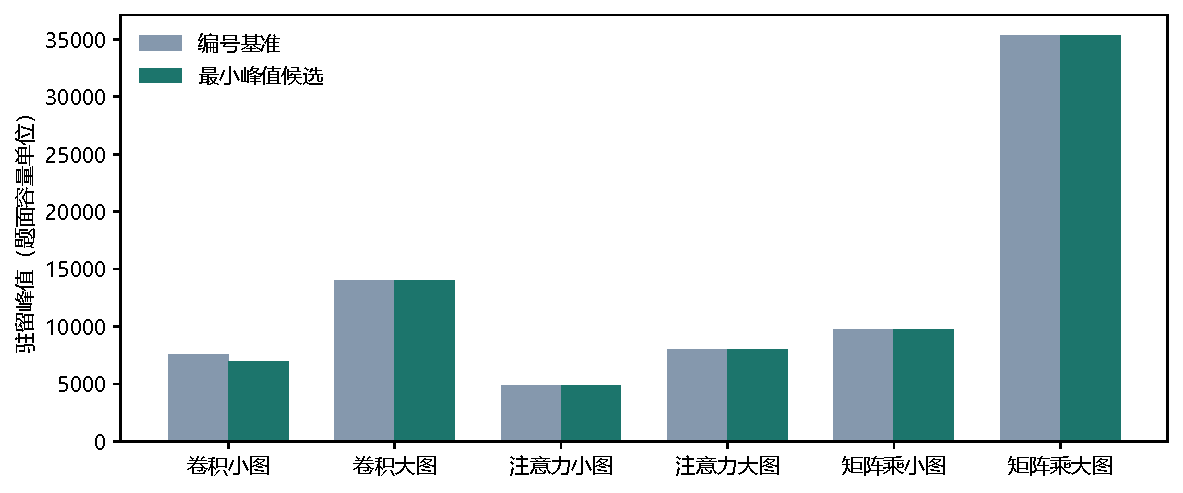
\includegraphics[width=.94\linewidth]{../figures/npu2025/peak.pdf}
\caption{生命周期收缩后的编号基准与选定候选的驻留峰值}\label{fig:peak}\end{figure}
卷积小图从 7560 降至 6984；其余五图未找到比收缩后的编号基准更好的峰值，因而保留基准。图\ref{fig:peak}反映的是本轮候选比较结果，不能据此认定其他图已达到理论下界。该现象也提示，输入编号可能已包含有利的局部组织，复杂启发式未必优于简单基准。

